\documentclass[a5paper]{letter}

% \usepackage{a5paper}

\usepackage[top=0.0cm, bottom=0.0cm, left=0.0cm, right=0.0cm]{geometry}
% gauche, haut, droite, bas, entete, ente2txt, pied, txt2pied
% \usepackage{vmargin}
% \setmarginsrb{0.00cm}{0.00cm}{0.00cm}{0.00cm}{0pt}{0pt}{0pt}{0pt}

\usepackage{tikz}
\usetikzlibrary{decorations.pathmorphing, shapes}
\usetikzlibrary{shapes.geometric, intersections, calc}
\usetikzlibrary{decorations.markings, arrows}

\begin{document}
	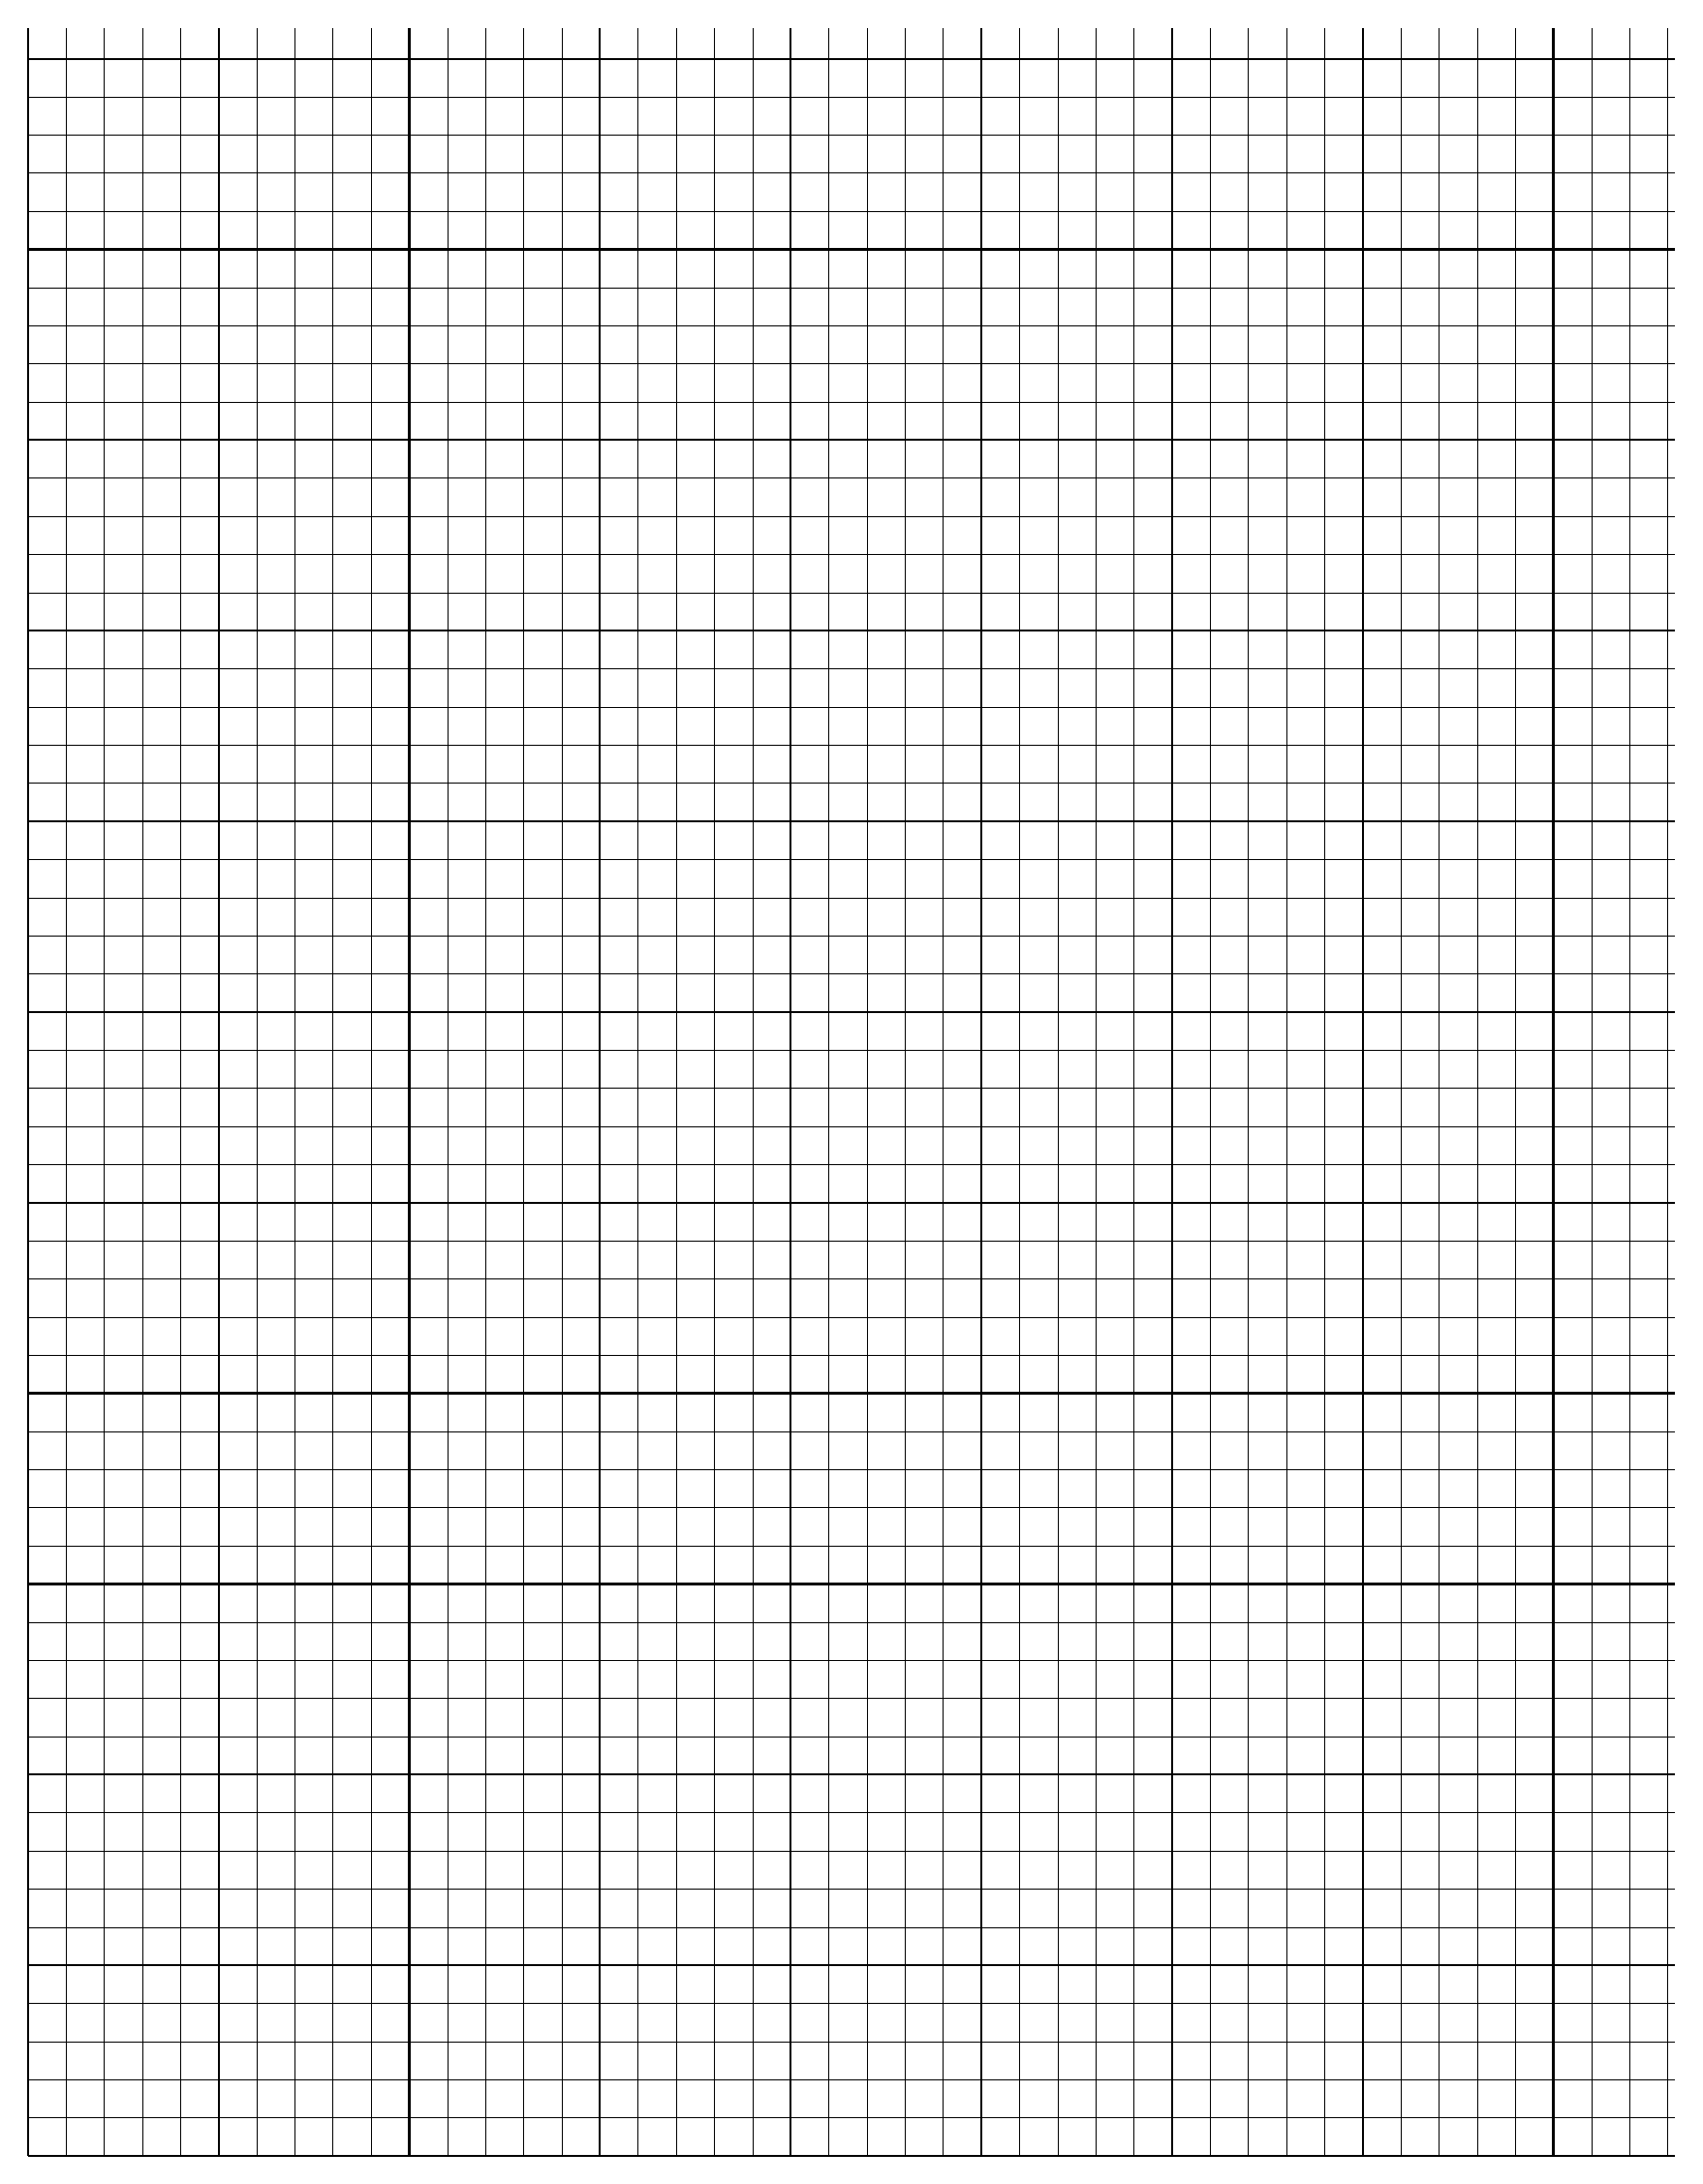
\begin{tikzpicture}
		\draw[thick] (0,0) grid[step=2.5] (\paperwidth,\paperheight-1);
		\draw[very thin] (0,0) grid[step=0.5] (\paperwidth,\paperheight-1);
	\end{tikzpicture}
\end{document}
